\documentclass[11pt,a4paper]{article}

% --- Packages for Typography & Layout ---
\usepackage[margin=1in]{geometry}
\usepackage[T1]{fontenc}
\usepackage[utf8]{inputenc}
\usepackage{lmodern}
\usepackage{microtype}
\usepackage{amsmath,amssymb,amsfonts,mathtools}
\usepackage{booktabs,array,tabularx,multirow}
\usepackage{xcolor}
\usepackage{enumitem}
\usepackage{titlesec}
\usepackage{caption,subcaption}
\usepackage{algorithm}
\usepackage{algpseudocode}

% --- TikZ & PGFPlots for Standalone Diagrams ---
\usepackage{tikz}
\usetikzlibrary{arrows.meta,positioning,shapes.geometric,shapes.misc,fit,calc,shadows,decorations.pathreplacing,trees}

% --- Modern Box Environments ---
\usepackage[skins,breakable]{tcolorbox}

% --- Hyperref Setup ---

% --- Missing Macros & Shorthands ---
\providecommand{\checkmark}{\ensuremath{\surd}}
\newcommand{\Valid}{\textsc{valid}}
\newcommand{\Causal}{\textsc{causal}}
\newcommand{\Action}{\textsc{actionable}}
\newcommand{\Usable}{\textsc{usable}}
\newcommand{\cac}{\textsc{cac}}
\newcommand{\dopart}[1]{\ensuremath{\mathrm{do}(#1)}}
\usepackage[hidelinks]{hyperref}
\hypersetup{
    colorlinks=true,
    linkcolor=teal!70!black,
    citecolor=blue!70!black,
    urlcolor=purple!70!black
}

% --- Color Palette (Modern Deep & Warm Tones) ---
\definecolor{parentdark}{RGB}{20, 35, 60}
\definecolor{parentheader}{RGB}{35, 65, 110}
\definecolor{branchdark}{RGB}{40, 80, 70}
\definecolor{branchheader}{RGB}{45, 120, 100}
\definecolor{codedark}{RGB}{60, 40, 75}
\definecolor{codeheader}{RGB}{110, 70, 140}
\definecolor{analogygold}{RGB}{180, 110, 20}
\definecolor{lightbg}{RGB}{248, 250, 252}
\definecolor{alertred}{RGB}{180, 40, 40}

% --- Custom Environments for Tree-and-Branch Structure ---
\newtcolorbox{parentconcept}[2][]{
    enhanced,
    breakable,
    colback=parentheader!5!white,
    colframe=parentheader,
    coltitle=white,
    fonttitle=\bfseries\large,
    title={$\blacktriangleright$ [PARENT CONCEPT] #2},
    attach boxed title to top left={yshift=-2mm, xshift=5mm},
    boxed title style={colback=parentheader, sharp corners},
    boxrule=1.2pt,
    arc=3mm,
    top=5mm,
    bottom=3mm,
    left=4mm,
    right=4mm,
    #1
}

\newtcolorbox{childbranch}[2][]{
    enhanced,
    breakable,
    colback=branchheader!4!white,
    colframe=branchheader!85!black,
    coltitle=white,
    fonttitle=\bfseries,
    title={$\hookrightarrow$ [BRANCH] #2},
    attach boxed title to top left={yshift=-2mm, xshift=8mm},
    boxed title style={colback=branchheader!85!black, rounded corners},
    boxrule=0.9pt,
    arc=2mm,
    top=4mm,
    bottom=3mm,
    left=5mm,
    right=4mm,
    #1
}

\newtcolorbox{codeanatomy}[2][]{
    enhanced,
    breakable,
    colback=codeheader!5!white,
    colframe=codeheader,
    coltitle=white,
    fonttitle=\bfseries\small,
    title={$\blacksquare$ [CODE ANATOMY] #2},
    attach boxed title to top left={yshift=-1.8mm, xshift=6mm},
    boxed title style={colback=codeheader, sharp corners},
    boxrule=0.8pt,
    arc=1.5mm,
    top=4mm,
    bottom=3mm,
    left=4mm,
    right=4mm,
    #1
}

\newtcolorbox{analogybox}[1][Real-World Intuition]{
    enhanced,
    colback=analogygold!6!white,
    colframe=analogygold,
    coltitle=white,
    fonttitle=\bfseries\small,
    title={$\bigstar$ [ANALOGY] #1},
    boxrule=0.8pt,
    arc=2mm,
    top=2mm, bottom=2mm, left=3mm, right=3mm
}

\newtcolorbox{warningbox}[1][Critical Failure Mode]{
    enhanced,
    colback=alertred!6!white,
    colframe=alertred,
    coltitle=white,
    fonttitle=\bfseries\small,
    title={$\triangle$ [FAILURE MODE] #1},
    boxrule=0.9pt,
    arc=2mm,
    top=2mm, bottom=2mm, left=3mm, right=3mm
}

% --- Custom Section Formatting ---
\titleformat{\section}{\Large\bfseries\color{parentheader}}{\thesection}{1em}{}[\titlerule]
\titleformat{\subsection}{\large\bfseries\color{branchheader}}{\thesubsection}{1em}{}
\titleformat{\subsubsection}{\normalsize\bfseries\color{parentdark}}{\thesubsubsection}{1em}{}

% --- Title Information ---
\title{\Huge\bfseries Causal Actionable Counterfactuals (CAC)\\[6pt]
\Large\color{parentheader} Architectural Master Reference \& Tree-and-Branch Codebase Guide}
\author{\textbf{Comprehensive System Deconstruction and Implementation Walkthrough}}
\date{\today}

\begin{document}

\maketitle

\begin{abstract}
\noindent
This document provides an exhaustive, multi-phase, tree-and-branch architectural deconstruction of the \textbf{Causal Actionable Counterfactuals (CAC)} repository (\texttt{cac-blackbox-to-action}). Traditional counterfactual algorithms (e.g., Wachter et al., DiCE) identify mathematical points in feature space that invert a black-box model's decision, but routinely prescribe advice that is physically impossible, economically irrational, or causally self-destructive. 
CAC re-conceptualizes algorithmic recourse from a \emph{point search} to an \emph{action search} ($\mathrm{do}(X_S = v_S)$) operating through a Structural Causal Model (SCM). 

\medskip\noindent
To make this complex mathematical, statistical, and software engineering system fully transparent, this guide is structured into \textbf{8 sequential phases}. Each phase employs a strict \textbf{Tree-and-Branch Pedagogical Layout}: high-level technical terms and formal theorems act as \textbf{Parent Concepts}, from which branch out \textbf{Intuitive Branches} (plain-English translations, real-world analogies, failure modes) and \textbf{Code Anatomy Branches} (exact file locations, class interfaces, mathematical formulas, and algorithmic routines). All architectural flowcharts, causal graphs, and algorithmic structures are natively rendered in standalone TikZ environments.
\end{abstract}

\tableofcontents
\newpage

% =========================================================================
% PHASE 1: THE RECOURSE CRISIS & THE RECOURSE TRILEMMA
% =========================================================================
\section{Phase 1: Conceptual Foundations \& The Recourse Trilemma}
\label{sec:phase1}

The field of Explainable Artificial Intelligence (XAI) was built on a foundational promise: when an automated decision system rejects a human applicant (for a bank loan, a job interview, or medical triage), it must provide an explanation that empowers the person to obtain a favorable outcome. This phase deconstructs why standard approaches fail and establishes the mathematical bedrock of CAC.

\subsection{Tree-and-Branch Overview: The Recourse Crisis}

\begin{center}
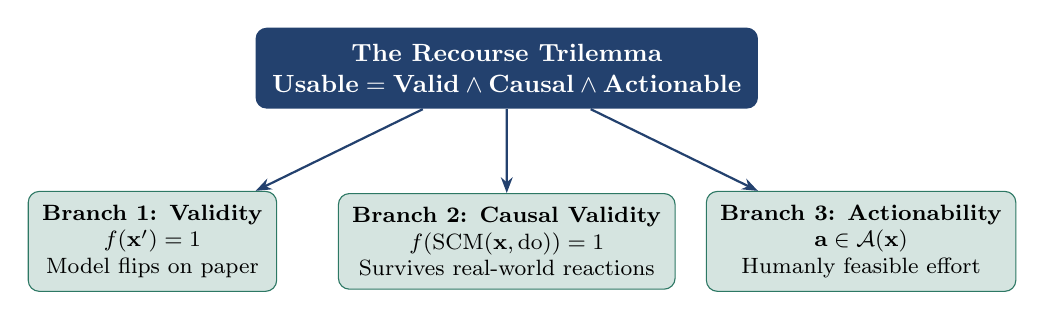
\begin{tikzpicture}[
    level distance=2.2cm,
    sibling distance=4.5cm,
    edge from parent/.style={draw=parentheader, -{Stealth[length=2mm]}, thick},
    parent_node/.style={rectangle, rounded corners, fill=parentheader, text=white, font=\bfseries\small, align=center, inner sep=6pt},
    child_node/.style={rectangle, rounded corners, fill=branchheader!20, draw=branchheader, text=black, font=\footnotesize, align=center, inner sep=5pt}
]
\node[parent_node] {The Recourse Trilemma\\$\text{Usable} = \text{Valid} \land \text{Causal} \land \text{Actionable}$}
    child { node[child_node] {\textbf{Branch 1: Validity}\\$f(\mathbf{x}') = 1$\\ Model flips on paper} }
    child { node[child_node] {\textbf{Branch 2: Causal Validity}\\$f(\mathrm{SCM}(\mathbf{x}, \mathrm{do})) = 1$\\ Survives real-world reactions} }
    child { node[child_node] {\textbf{Branch 3: Actionability}\\$\mathbf{a} \in \mathcal{A}(\mathbf{x})$\\ Humanly feasible effort} };
\end{tikzpicture}
\end{center}

\begin{parentconcept}{The Fundamental Trilemma of Counterfactual Recourse}
Traditional counterfactual generation frames recourse as an optimization problem over input vectors:
\begin{equation}
\mathbf{x}^* = \arg\min_{\mathbf{x}'} \mathcal{D}(\mathbf{x}, \mathbf{x}') \quad \text{subject to} \quad f(\mathbf{x}') = 1
\end{equation}
where $f: \mathcal{X} \to \{0, 1\}$ is the frozen black-box classifier, $\mathbf{x} \in \mathcal{X}$ is the rejected factual instance, and $\mathcal{D}(\cdot)$ is a distance metric (e.g., $L_1$ or $L_2$). CAC establishes that this framing is fundamentally flawed because it conflates three distinct and frequently contradictory properties:
\begin{enumerate}[leftmargin=1.5em]
    \item \textbf{Validity ($\Valid$):} Does the proposed state $\mathbf{x}'$ cross the decision boundary of $f$ in isolation?
    \item \textbf{Causal Validity ($\Causal$):} If the applicant executes the actions that lead to $\mathbf{x}'$, does the resulting state $\mathbf{x}^{\text{replayed}}$ generated by the laws of nature and economics still satisfy $f(\mathbf{x}^{\text{replayed}}) = 1$?
    \item \textbf{Actionability ($\Action$):} Does the change respect human constraints (e.g., non-negative time flow, immutable protected attributes, monotonicity, and cognitive bandwidth)?
\end{enumerate}
\textbf{The Primary Endpoint:} An explanation provides \textbf{Usable Recourse ($\Usable$)} if and only if it is simultaneously \emph{Causally Valid} and \emph{Actionable}:
\begin{equation}
\Usable(\mathbf{x}, \mathbf{a}) \iff \Causal(\mathbf{x}, \mathbf{a}) \land \Action(\mathbf{x}, \mathbf{a})
\end{equation}
\end{parentconcept}

\begin{childbranch}{Point Search vs. Action Search}
\textbf{What does this mean in plain language?}
Traditional algorithms treat a human being like a cursor on a computer screen. They slide feature values across a coordinate grid until the model's output switches from ``Rejected'' to ``Approved''. This is a \emph{Point Search}: the algorithm outputs a dream state $\mathbf{x}'$ without asking how anybody gets there.

\medskip\noindent
In contrast, CAC conducts an \textbf{Action Search}. It searches over a set of real-world interventions:
\begin{equation}
\mathbf{a} = \mathrm{do}(X_1 = v_1, X_2 = v_2, \dots)
\end{equation}
Instead of wishing for an arbitrary destination, CAC searches for the \emph{levers} a person can pull, and then uses a causal simulator (the SCM) to project where those levers will actually land them.
\end{childbranch}

\begin{analogybox}[The Thermostat Analogy]
Imagine you want your living room to feel warmer.
\begin{itemize}[leftmargin=1.2em]
    \item \textbf{Point Search (Acausal):} Tells you: \emph{``Set the thermometer on the wall to 72$^\circ$F, and also keep the air temperature at 72$^\circ$F, while opening the freezer.''} It treats every reading as independent. If you open the freezer, the air cools, the thermostat drops, and you freeze.
    \item \textbf{Action Search (CAC):} Tells you: \emph{``Turn the furnace knob to 72$^\circ$F.''} It models the consequence: the furnace ignites, hot air blows through the ducts, the room warms up, and the thermometer reading naturally follows.
\end{itemize}
\end{analogybox}

\begin{warningbox}[The Dangerous Optical Illusion of 100\% Validity]
Across the benchmark datasets (Adult, German Credit, HELOC, Diabetes), existing algorithms like Wachter et al. and DiCE achieve \textbf{100\% Validity}. To an auditor looking only at paper benchmarks, they appear perfect. 
However, once their suggestions are audited through realistic structural equations, their \textbf{Usable Recourse rate collapses to between 13\% and 32\%}! 
They tell applicants to decrease work experience, increase age, or expect income to quadruple without education changing. 100\% mathematical validity is an optical illusion that masks catastrophic real-world failure.
\end{warningbox}

\begin{codeanatomy}{Repository Mapping: Metrics \& Trilemma Definitions}
\begin{itemize}[leftmargin=1.2em]
    \item \textbf{Audit Definitions:} Defined in \texttt{src/evaluation/metrics.py} (\texttt{BASE\_COLUMNS}, \texttt{evaluate()}).
    \item \textbf{Usable Rate Formulation:} Located in \texttt{src/evaluation/feasibility.py} and computed in \texttt{experiments/02\_compare\_methods.py}.
    \item \textbf{Audit Functions:}
    \begin{itemize}
        \item \texttt{valid}: $\mathbb{I}[f(\mathbf{x}') = y_{\text{target}}]$
        \item \texttt{causal\_valid}: $\mathbb{I}[f(\mathrm{FCM}.\text{counterfactual}(\mathbf{x}, \mathbf{a})) = y_{\text{target}}]$
        \item \texttt{feasible}: Respects immutability, directionality, and action budget.
        \item \texttt{usable}: \texttt{causal\_valid} $\land$ \texttt{feasible}.
    \end{itemize}
\end{itemize}
\end{codeanatomy}

% =========================================================================
% PHASE 2: THE DATA & SCHEMA LAYER (src/data/)
% =========================================================================
\newpage
\section{Phase 2: The Data \& Schema Layer (\texttt{src/data/})}
\label{sec:phase2}

Machine learning pipelines often treat tabular columns as generic floating-point arrays. In recourse, this causes immediate failure: columns represent physical entities with strict rules of nature (e.g., age cannot decrease, educational degrees are discrete ladders, marital status cannot be averaged). The data layer in CAC enforces a rigorous declarative schema.

\subsection{Tree-and-Branch Overview: Data Architecture}

\begin{center}
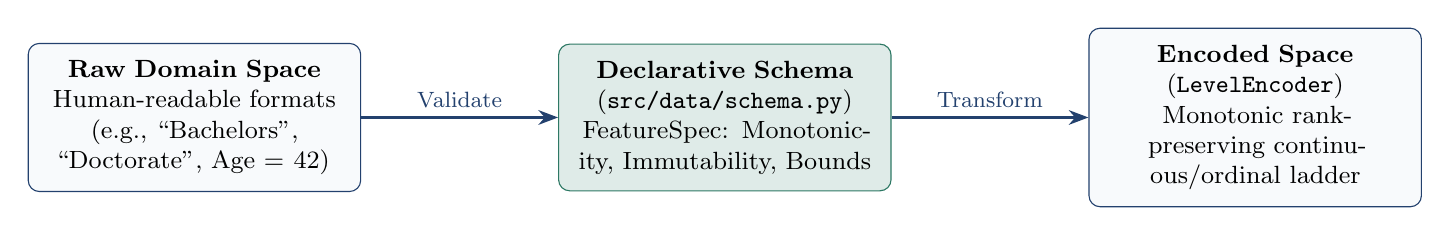
\begin{tikzpicture}[
    node distance=1.5cm and 2.5cm,
    box/.style={rectangle, rounded corners, draw=parentheader, fill=lightbg, font=\small, align=center, inner sep=6pt, text width=3.8cm},
    actionbox/.style={rectangle, rounded corners, draw=branchheader, fill=branchheader!15, font=\small, align=center, inner sep=6pt, text width=3.8cm},
    arrow/.style={-{Stealth[length=2.5mm]}, thick, color=parentheader}
]
\node[box] (raw) {\textbf{Raw Domain Space}\\ Human-readable formats\\(e.g., ``Bachelors'', ``Doctorate'', Age $= 42$)};
\node[actionbox, right=of raw] (schema) {\textbf{Declarative Schema}\\(\texttt{src/data/schema.py})\\ FeatureSpec: Monotonicity, Immutability, Bounds};
\node[box, right=of schema] (enc) {\textbf{Encoded Space}\\(\texttt{LevelEncoder})\\ Monotonic rank-preserving continuous/ordinal ladder};

\draw[arrow] (raw) -- node[above, font=\footnotesize] {Validate} (schema);
\draw[arrow] (schema) -- node[above, font=\footnotesize] {Transform} (enc);
\end{tikzpicture}
\end{center}

\begin{parentconcept}{Declarative Schema Contract (\texttt{src/data/schema.py})}
The schema forms the binding legal contract between four decoupled pipeline layers:
\begin{equation}
\text{Data Layer} \iff \text{SCM Layer} \iff \text{Cost Layer} \iff \text{Search Layer}
\end{equation}
Each feature is encapsulated in a \texttt{FeatureSpec} dataclass defining:
\begin{itemize}[leftmargin=1.5em]
    \item \texttt{name}: Feature identifier string.
    \item \texttt{kind}: One of \texttt{\{"numeric", "ordinal", "categorical", "binary"\}}.
    \item \texttt{levels}: Ordered tuple of discrete levels (e.g., \texttt{("HS-grad", "Some-college", "Bachelors", ...)}).
    \item \texttt{bounds}: Strict closed interval $[a, b]$ in encoded space.
    \item \texttt{manipulable}: Boolean flag indicating whether human agency can directly alter this variable.
    \item \texttt{monotone}: Directional constraint: \texttt{"any"}, \texttt{"increase"}, or \texttt{"decrease"}.
    \item \texttt{protected}: Sensitive attribute marker (for fairness auditing).
\end{itemize}
\end{parentconcept}

\begin{childbranch}{Why Standard Encoders Destroy Causal Recourse}
\textbf{The Technical Pitfall:}
Standard tools like Scikit-Learn's \texttt{LabelEncoder} assign integer codes alphabetically. For education:
\begin{equation}
\text{``Assoc-acdm''} \to 0, \quad \text{``Bachelors''} \to 1, \quad \text{``Doctorate''} \to 2, \quad \text{``HS-grad''} \to 3
\end{equation}
Under this naive encoding, moving from High School ($3$) to Bachelors ($1$) is encoded as a \emph{negative step} of $-2$. If an optimizer enforces ``education must increase'', it will forbid a High School graduate from obtaining a Bachelor's degree, while encouraging them to downgrade to an Associate's degree!

\medskip\noindent
\textbf{The Solution: \texttt{LevelEncoder}}
Located in \texttt{src/data/preprocess.py}, CAC's custom \texttt{LevelEncoder} constructs a rank-preserving mapping where numerical values strictly mirror natural ordinal progression. If an intervention shifts encoded education from $2.0 \to 4.0$, it is guaranteed to represent positive educational attainment.
\end{childbranch}

\begin{parentconcept}{The Dual-Space Architecture}
The repository strictly isolates two representations of every record:
\begin{enumerate}[leftmargin=1.5em]
    \item \textbf{Raw Space $\mathcal{X}_{\text{raw}}$:} Human-interpretable tables (DataFrames with strings, dates, and unscaled dollars). This space is used exclusively for loading, final report presentation, and user studies.
    \item \textbf{Encoded Space $\mathcal{X}_{\text{enc}}$:} Normalized floating-point vectors $\mathbf{x} \in \mathbb{R}^d$ where discrete features are mapped to $[0, L-1]$ and continuous features are scaled. The SCM, black-box classifiers, cost functions, and evolutionary search algorithms operate \emph{exclusively} in this space.
\end{enumerate}
\end{parentconcept}

\begin{table}[htbp]
\centering
\caption{The Benchmark Datasets Evaluated in the CAC Codebase}
\label{tab:datasets_overview}
\small
\begin{tabularx}{\textwidth}{lcccccX}
\toprule
\textbf{Dataset} & \textbf{Nodes} & \textbf{Edges} & \textbf{Manipulable} & \textbf{Target Meaning} & \textbf{Key Characteristics} \\
\midrule
\textbf{Adult Income} & 10 & 25 & 6 & Income $> \$50\text{k}$ & Complex social mediators; demographic constraints. \\
\textbf{German Credit} & 11 & 37 & 7 & Good Credit & Dense inter-correlation; financial risk features. \\
\textbf{HELOC} & 12 & 28 & 8 & Favorable Repayment & High-dimensional risk indices; financial credit lines. \\
\textbf{Pima Diabetes} & 8 & 14 & 5 & No Diabetes & Inverted clinical label ($1 - \text{Outcome}$); non-linear SCM. \\
\textbf{synth\_reach} & 6 & 7 & 4 & Analytic Acceptance & Known ground truth; every rejection has feasible recourse. \\
\textbf{synth\_block} & 6 & 7 & 3 & Analytic Acceptance & Known ground truth; contains structural bottlenecks. \\
\bottomrule
\end{tabularx}
\end{table}

\begin{codeanatomy}{Repository Mapping: Data Loaders and Schema Definitions}
\begin{itemize}[leftmargin=1.2em]
    \item \texttt{src/data/schema.py}: Declares \texttt{FeatureSpec}, \texttt{DatasetSpec}, and helper methods (\texttt{encoded\_bounds()}, \texttt{is\_discrete}).
    \item \texttt{src/data/preprocess.py}: Implements \texttt{LevelEncoder}, \texttt{Transformer}, and \texttt{build\_dataset()} for deterministic splits ($70\%$ train, $15\%$ val, $15\%$ test).
    \item \texttt{src/data/load\_*.py}: Dataset-specific loaders:
    \begin{itemize}
        \item \texttt{load\_adult.py}: Cleans census data, defines 10 core nodes.
        \item \texttt{load\_diabetes.py}: Inverts target so $1 = \text{healthy}$; strips class-conditional leakage in Insulin/SkinThickness.
        \item \texttt{load\_synth\_reach.py} \& \texttt{load\_synth\_block.py}: Procedural generation with ground-truth causal mechanisms.
    \end{itemize}
\end{itemize}
\end{codeanatomy}

% =========================================================================
% PHASE 3: THE OPAQUE BLACK-BOX MODELS (src/model/)
% =========================================================================
\newpage
\section{Phase 3: The Opaque Black-Box Models (\texttt{src/model/})}
\label{sec:phase3}

Many counterfactual methods in the literature assume white-box access: they backpropagate gradients directly through the neural network weights $\nabla_{\mathbf{x}} f(\mathbf{x})$ to guide the search. In real-world enterprise deployments, this assumption is invalid. Banks, healthcare providers, and insurance companies deploy proprietary models behind rate-limited prediction endpoints.

\subsection{Tree-and-Branch Overview: Black-Box Architecture}

\begin{center}
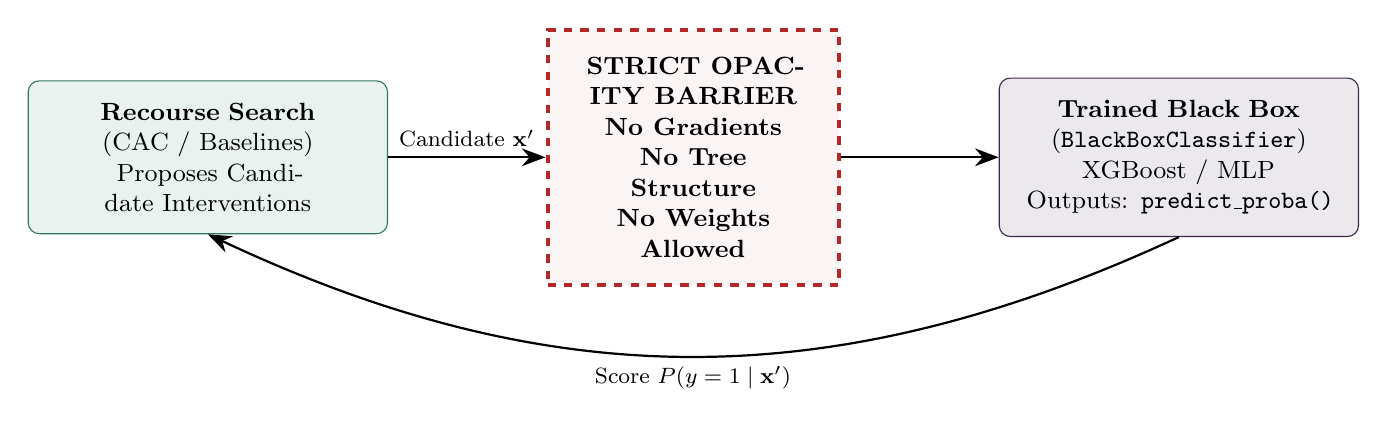
\begin{tikzpicture}[
    box/.style={rectangle, rounded corners, draw=codedark, fill=codedark!10, font=\small, align=center, inner sep=8pt, text width=4cm},
    barrier/.style={rectangle, draw=alertred, dashed, line width=1.5pt, fill=alertred!5, font=\bfseries\small, align=center, inner sep=10pt, text width=3cm},
    client/.style={rectangle, rounded corners, draw=branchheader, fill=branchheader!10, font=\small, align=center, inner sep=8pt, text width=4cm}
]
\node[client] (search) {\textbf{Recourse Search}\\(CAC / Baselines)\\ Proposes Candidate Interventions};
\node[barrier, right=2cm of search] (wall) {\textbf{STRICT OPACITY BARRIER}\\ No Gradients\\ No Tree Structure\\ No Weights Allowed};
\node[box, right=2cm of wall] (model) {\textbf{Trained Black Box}\\(\texttt{BlackBoxClassifier})\\ XGBoost / MLP\\ Outputs: \texttt{predict\_proba()}};

\draw[-{Stealth[length=3mm]}, thick] (search.east) -- node[above, font=\footnotesize] {Candidate $\mathbf{x}'$} (wall.west);
\draw[-{Stealth[length=3mm]}, thick] (wall.east) -- (model.west);
\draw[{Stealth[length=3mm]}-, thick] (search.south) to[bend right=25] node[below, font=\footnotesize] {Score $P(y=1 \mid \mathbf{x}')$} (model.south);
\end{tikzpicture}
\end{center}

\begin{parentconcept}{The Strict Opacity Contract (\texttt{src/model/blackbox.py})}
CAC models black boxes under the most adversarial realistic setting:
\begin{equation}
f: \mathbb{R}^d \to [0, 1] \quad \text{exposes ONLY} \quad \texttt{predict}(\mathbf{x}) \;\text{and}\; \texttt{predict\_proba}(\mathbf{x})
\end{equation}
The black box is wrapped in a strict interface class \texttt{BlackBoxClassifier}. It explicitly prevents methods from inspecting:
\begin{itemize}[leftmargin=1.5em]
    \item Tree structures, leaf values, or split points (in XGBoost).
    \item Layer weights, activations, or backpropagated gradients (in MLP).
    \item Global or local feature importances (e.g., SHAP, permutation scores).
\end{itemize}
Every candidate query is counted through an internal audit counter to ensure cost accounting across methods is rigorously matched.
\end{parentconcept}

\begin{childbranch}{Why Piecewise-Constant Trees Break Gradients}
\textbf{The Mathematical Reality:}
Gradient boosted decision trees (XGBoost) partition $\mathbb{R}^d$ into hyper-rectangles:
\begin{equation}
f_{\text{XGB}}(\mathbf{x}) = \sum_{t=1}^T w_{q_t(\mathbf{x})}
\end{equation}
where $q_t(\mathbf{x})$ maps instance $\mathbf{x}$ to a tree leaf index, and $w$ is the scalar leaf weight. 
Inside any hyper-rectangle, the output is a constant flat plateau. Therefore:
\begin{equation}
\nabla_{\mathbf{x}} f_{\text{XGB}}(\mathbf{x}) = \mathbf{0} \quad \text{almost everywhere!}
\end{equation}
Gradient-based recourse algorithms (like vanilla Wachter et al.) get stuck instantly because the derivative gives zero direction. Finite-difference approximations either land on zero or cross a step discontinuity. A gradient-free optimization engine is mathematically required.
\end{childbranch}

\begin{table}[htbp]
\centering
\caption{Held-Out Generalization Performance of Primary Black Boxes}
\label{tab:blackbox_perf}
\small
\begin{tabular}{lcccccc}
\toprule
\textbf{Dataset} & \textbf{Model Type} & \textbf{Accuracy} & \textbf{ROC-AUC} & \textbf{Macro F1} & \textbf{Brier Score} \\
\midrule
\textbf{Adult Income} & XGBoost & $0.871$ & $0.924$ & $0.812$ & $0.093$ \\
\textbf{German Credit} & XGBoost & $0.780$ & $0.814$ & $0.715$ & $0.154$ \\
\textbf{HELOC} & XGBoost & $0.732$ & $0.801$ & $0.728$ & $0.178$ \\
\textbf{Pima Diabetes} & XGBoost & $0.793$ & $0.849$ & $0.761$ & $0.141$ \\
\bottomrule
\end{tabular}
\end{table}

\begin{codeanatomy}{Repository Mapping: Model Training \& Wrapping}
\begin{itemize}[leftmargin=1.2em]
    \item \texttt{src/model/blackbox.py}: Defines \texttt{BlackBoxClassifier}, holding the scikit-learn/XGBoost pipeline, query counters, and calibration wrappers.
    \item \texttt{src/model/train.py}: Script that trains black boxes across datasets using 5-fold cross-validation and hyperparameter grids, serializing trained artifacts to \texttt{models/blackbox\_<dataset>\_<kind>.joblib}.
    \item \texttt{experiments/01\_train\_blackbox.py}: Command-line entry point to train and validate all black boxes deterministically.
\end{itemize}
\end{codeanatomy}

% =========================================================================
% PHASE 4: STRUCTURAL & FUNCTIONAL CAUSAL MODELS (src/scm/)
% =========================================================================
\newpage
\section{Phase 4: Structural \& Functional Causal Models (\texttt{src/scm/})}
\label{sec:phase4}

The centerpiece of CAC is the recognition that the world has physical, sociological, and economic structure. Changing one feature causes ripple effects throughout dependent downstream variables. This phase formalizes how causal graphs are defined, validated, and computed.

\subsection{Tree-and-Branch Overview: Causal Engine}

\begin{center}
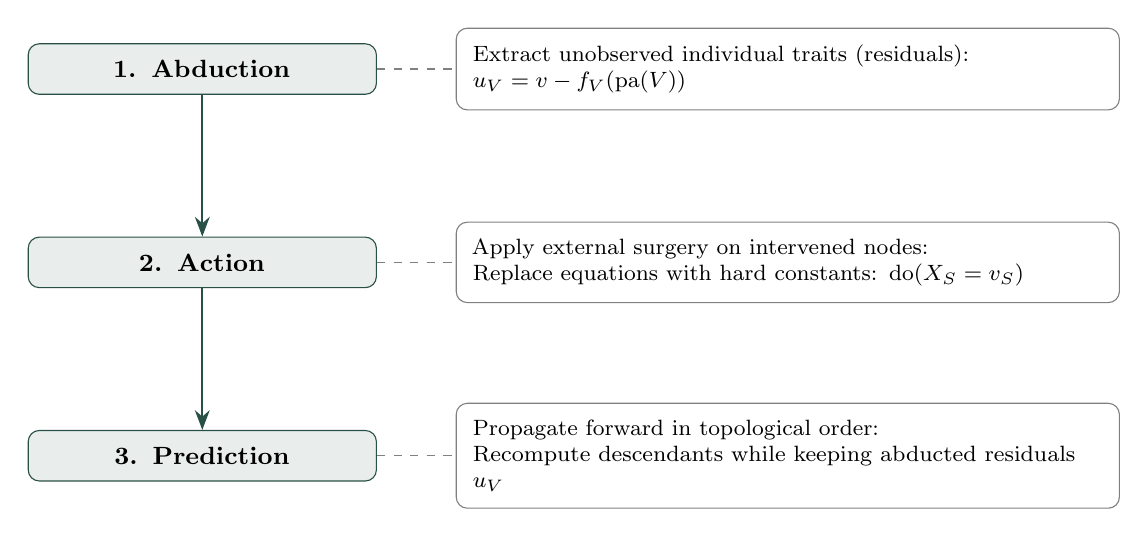
\begin{tikzpicture}[
    node distance=1.8cm,
    step_node/.style={rectangle, rounded corners, draw=branchdark, fill=branchdark!10, font=\bfseries\small, align=center, inner sep=6pt, text width=4cm},
    detail_node/.style={rectangle, rounded corners, draw=gray, fill=white, font=\footnotesize, align=left, inner sep=6pt, text width=8cm},
    arrow/.style={-{Stealth[length=2.5mm]}, thick, color=branchdark}
]
\node[step_node] (step1) {1. Abduction};
\node[detail_node, right=1cm of step1] (d1) {Extract unobserved individual traits (residuals):\\$u_V = v - f_V(\mathrm{pa}(V))$};

\node[step_node, below=of step1] (step2) {2. Action};
\node[detail_node, right=1cm of step2] (d2) {Apply external surgery on intervened nodes:\\ Replace equations with hard constants: $\mathrm{do}(X_S = v_S)$};

\node[step_node, below=of step2] (step3) {3. Prediction};
\node[detail_node, right=1cm of step3] (d3) {Propagate forward in topological order:\\ Recompute descendants while keeping abducted residuals $u_V$};

\draw[arrow] (step1) -- (step2);
\draw[arrow] (step2) -- (step3);
\draw[dashed, color=gray] (step1) -- (d1);
\draw[dashed, color=gray] (step2) -- (d2);
\draw[dashed, color=gray] (step3) -- (d3);
\end{tikzpicture}
\end{center}

\begin{parentconcept}{Pearl's Structural Causal Models (\texttt{src/scm/define\_scm.py})}
A Structural Causal Model (SCM) $\mathcal{M}$ is defined as a 4-tuple $\langle U, V, \mathcal{F}, P(U) \rangle$:
\begin{itemize}[leftmargin=1.5em]
    \item $U$: Set of exogenous (unobserved background) variables.
    \item $V$: Set of endogenous (observed system) variables.
    \item $\mathcal{F}$: Set of structural deterministic equations $V_i = f_i(\mathrm{Pa}(V_i), U_i)$, where $\mathrm{Pa}(V_i) \subseteq V \setminus \{V_i\}$ are the direct causal parents of $V_i$.
    \item $P(U)$: Joint probability distribution over the exogenous variables.
\end{itemize}
In CAC, the causal graph $\mathcal{G} = (V, E)$ is represented as a \texttt{networkx.DiGraph}. Topological ordering guarantees that causes precede effects:
\begin{equation}
\text{Topological Sort: } \pi = (V_{(1)}, V_{(2)}, \dots, V_{(d)}) \quad \text{such that } (V_i \to V_j) \implies \pi(i) < \pi(j)
\end{equation}
\end{parentconcept}

\begin{childbranch}{The 3-Step Counterfactual Engine (\texttt{src/scm/fcm.py})}
\textbf{How does Pearl's counterfactual engine work in plain English?}
When someone asks: \emph{``What would have happened if I had completed college?''}, they are not asking what happens to an average stranger. They are asking what happens to \textbf{them}, with their specific work ethic, natural talents, and life circumstances preserved.

\medskip\noindent
Pearl's counterfactual algorithm executes this in three distinct steps:
\begin{enumerate}[leftmargin=1.5em]
    \item \textbf{Step 1: Abduction (Diagnosing the Person's Uniqueness):}
    We observe the factual applicant $\mathbf{x}$. Using the structural equation $V_i = f_i(\mathrm{Pa}_i) + U_i$, we compute their specific background residual:
    \begin{equation}
    u_i = v_i - f_i(\mathrm{pa}_i)
    \end{equation}
    If the applicant works 50 hours a week, but the average person with their education works 40 hours, their abducted residual is $u_{\text{hours}} = +10$. They are an intrinsically hard worker!
    \item \textbf{Step 2: Action (Performing the Intervention):}
    We apply the applicant's chosen action: $\mathrm{do}(\text{Education} = \text{Bachelors})$. We sever the incoming edges to Education and lock it to its new value.
    \item \textbf{Step 3: Prediction (Propagating Consequences):}
    We recalculate all downstream descendants (e.g., Occupation, Capital Gains) along the causal DAG. Critically, we \textbf{reuse the abducted residual} $u_{\text{hours}} = +10$. Their updated work hours become:
    \begin{equation}
    v_{\text{hours}}^{\text{new}} = f_{\text{hours}}(\text{Bachelors}) + u_{\text{hours}} = 45 + 10 = 55\text{ hours}
    \end{equation}
\end{enumerate}
\end{childbranch}

\begin{figure}[htbp]
\centering
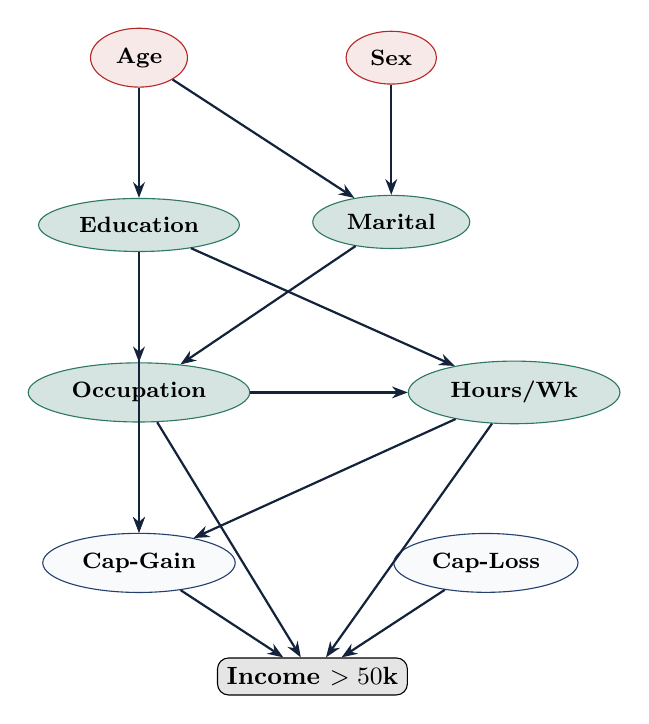
\begin{tikzpicture}[
    node distance=1.4cm and 2.0cm,
    var/.style={ellipse, draw=parentheader, fill=lightbg, font=\bfseries\footnotesize, align=center, inner sep=4pt},
    manip/.style={ellipse, draw=branchheader, fill=branchheader!20, font=\bfseries\footnotesize, align=center, inner sep=4pt},
    prot/.style={ellipse, draw=alertred, fill=alertred!10, font=\bfseries\footnotesize, align=center, inner sep=4pt},
    edge/.style={-{Stealth[length=2mm]}, thick, color=parentdark}
]
% Nodes
\node[prot] (age) {Age};
\node[prot, right=of age] (sex) {Sex};
\node[manip, below=of age] (edu) {Education};
\node[manip, below=of sex] (mar) {Marital};
\node[manip, below=of edu] (occ) {Occupation};
\node[manip, right=of occ] (hrs) {Hours/Wk};
\node[var, below=of occ] (gain) {Cap-Gain};
\node[var, right=of gain] (loss) {Cap-Loss};
\node[rectangle, rounded corners, draw=black, fill=gray!20, font=\bfseries\small, below=1.2cm of $(gain)!0.5!(loss)$] (target) {Income $> 50\text{k}$};

% Edges
\draw[edge] (age) -- (edu);
\draw[edge] (age) -- (mar);
\draw[edge] (sex) -- (mar);
\draw[edge] (edu) -- (occ);
\draw[edge] (edu) -- (hrs);
\draw[edge] (mar) -- (occ);
\draw[edge] (occ) -- (hrs);
\draw[edge] (occ) -- (gain);
\draw[edge] (edu) -- (gain);
\draw[edge] (hrs) -- (gain);
\draw[edge] (hrs) -- (target);
\draw[edge] (gain) -- (target);
\draw[edge] (loss) -- (target);
\draw[edge] (occ) -- (target);
\end{tikzpicture}
\caption{The Causal Directed Acyclic Graph (DAG) for the Adult Census Dataset. Green nodes represent manipulable levers; red nodes denote immutable protected attributes.}
\label{fig:adult_dag}
\end{figure}

\begin{parentconcept}{Fitting Heterogeneous Structural Equations (\texttt{src/scm/fcm.py})}
Real datasets contain mixed data types. In CAC, the Functional Causal Model (\texttt{FCM}) fits equations on the training split using non-linear gradient boosting:
\begin{itemize}[leftmargin=1.5em]
    \item \textbf{Continuous \& Ordinal Nodes:} Modeled using Additive Noise Models (ANM):
    \begin{equation}
    V = f_V(\mathrm{Pa}(V)) + U_V, \quad f_V \sim \texttt{HistGradientBoostingRegressor}
    \end{equation}
    \item \textbf{Categorical \& Discrete Nodes:} Modeled using conditional probability distributions:
    \begin{equation}
    P(V = k \mid \mathrm{Pa}(V)) \sim \texttt{HistGradientBoostingClassifier}
    \end{equation}
    Abduction on discrete nodes maps the observed category to a uniform quantile interval $u_V \in [F(k-1 \mid \mathrm{pa}), F(k \mid \mathrm{pa})]$, which is coupled to predict counterfactual transitions deterministically.
\end{itemize}
\end{parentconcept}

\begin{codeanatomy}{Repository Mapping: SCM \& FCM Engines}
\begin{itemize}[leftmargin=1.2em]
    \item \texttt{src/scm/define\_scm.py}: Loads \texttt{data/scm/<dataset>\_scm.json}, builds \texttt{networkx.DiGraph}, verifies acyclicity, and assigns effort multipliers.
    \item \texttt{src/scm/fcm.py}: Contains the \texttt{FCM} class:
    \begin{itemize}
        \item \texttt{fit(X)}: Fits regression and classification models for each equation.
        \item \texttt{abduct(x)}: Extracts residual matrix $U$.
        \item \texttt{counterfactual(x, actions)}: Executes the 3-step Pearlian counterfactual pass.
    \end{itemize}
    \item \texttt{src/scm/validate\_scm.py}: Validates asserted edges via linear and non-linear regression $R^2$ tests, saving results to \texttt{paper/tables/scm\_validation.tex}.
\end{itemize}
\end{codeanatomy}

% =========================================================================
% PHASE 5: THE COST & ADMISSIBILITY FRAMEWORK (src/cost/)
% =========================================================================
\newpage
\section{Phase 5: The Cost \& Admissibility Framework (\texttt{src/cost/})}
\label{sec:phase5}

In optimization, algorithms minimize whatever loss function they are given. If cost is poorly formulated, the optimizer cheats: it suggests small fractional shifts across twenty features, or sets age backwards by 6 months. CAC formulates a 4-tier cost framework.

\subsection{Tree-and-Branch Overview: Cost Architecture}

\begin{center}
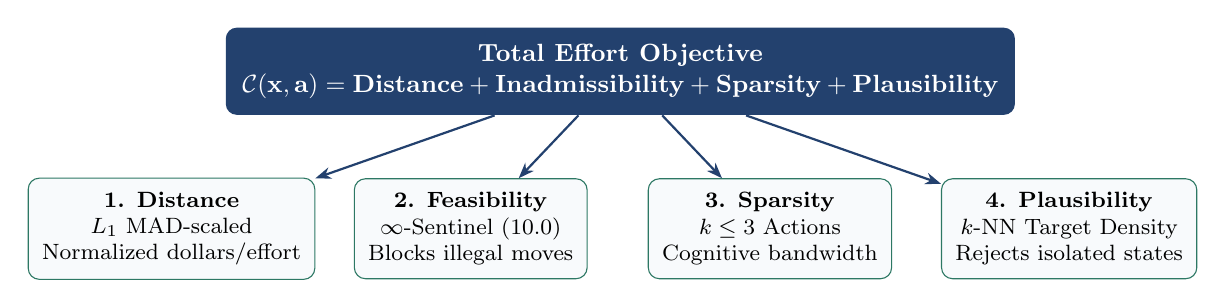
\begin{tikzpicture}[
    level distance=2.0cm,
    sibling distance=3.8cm,
    edge from parent/.style={draw=parentheader, -{Stealth[length=2mm]}, thick},
    pnode/.style={rectangle, rounded corners, fill=parentheader, text=white, font=\bfseries\small, align=center, inner sep=6pt},
    cnode/.style={rectangle, rounded corners, fill=lightbg, draw=branchheader, font=\footnotesize, align=center, inner sep=5pt}
]
\node[pnode] {Total Effort Objective\\$\mathcal{C}(\mathbf{x}, \mathbf{a}) = \text{Distance} + \text{Inadmissibility} + \text{Sparsity} + \text{Plausibility}$}
    child { node[cnode] {\textbf{1. Distance}\\$L_1$ MAD-scaled\\ Normalized dollars/effort} }
    child { node[cnode] {\textbf{2. Feasibility}\\$\infty$-Sentinel ($10.0$)\\ Blocks illegal moves} }
    child { node[cnode] {\textbf{3. Sparsity}\\$k \le 3$ Actions\\ Cognitive bandwidth} }
    child { node[cnode] {\textbf{4. Plausibility}\\$k$-NN Target Density\\ Rejects isolated states} };
\end{tikzpicture}
\end{center}

\begin{parentconcept}{The 4-Component Cost Formulation (\texttt{src/cost/cost\_functions.py})}
The total cost of proposing an intervention $\mathbf{a} = \mathrm{do}(X_S = v_S)$ on factual instance $\mathbf{x}$ is defined as:
\begin{equation}
\mathrm{Cost}(\mathbf{x}, \mathbf{a}) = \sum_{j \in S} c_j \cdot \frac{|v_j - x_j|}{\mathrm{MAD}_j} + \mathrm{Penalty}_{\text{inadmissible}}(\mathbf{x}, \mathbf{a})
\end{equation}
where:
\begin{itemize}[leftmargin=1.5em]
    \item $\mathrm{MAD}_j = \mathrm{median}(|X_j - \mathrm{median}(X_j)|)$: Median Absolute Deviation, which provides robust feature normalization immune to heavy-tailed outliers.
    \item $c_j \in [0.1, 10.0]$: Feature-specific effort multiplier assigned in the SCM schema (e.g., changing Education has a higher multiplier than changing Work Hours).
    \item $\mathrm{Penalty}_{\text{inadmissible}}$: Evaluates to $\infty$ (represented by sentinel $10.0$) if:
    \begin{enumerate}
        \item Feature $j$ is marked non-manipulable (\texttt{manipulable = False}).
        \item The change violates monotonicity (e.g., decreasing education or decreasing age).
        \item The intervention exceeds the maximum action sparsity budget ($|S| > k_{\max}$, where $k_{\max} = 3$).
    \end{enumerate}
\end{itemize}
\end{parentconcept}

\begin{childbranch}{Action Cost vs. State Cost}
\textbf{A Crucial Conceptual Distinction:}
Standard recourse methods evaluate the distance between the starting state $\mathbf{x}$ and the proposed counterfactual $\mathbf{x}'$. This is \textbf{State Cost}:
\begin{equation}
\mathrm{Cost}_{\text{state}} = \mathcal{D}(\mathbf{x}, \mathbf{x}')
\end{equation}
CAC reveals that this penalizes applicants unfairly! 

\medskip\noindent
\textbf{The Reality:}
If an applicant goes back to school and earns an MBA, their subsequent income increases and their job seniority rises. Under an acausal cost model, the applicant is penalized for their own pay raise! 
CAC measures \textbf{Action Cost}:
\begin{equation}
\mathrm{Cost}_{\text{action}} = \sum_{j \in S} \mathrm{cost}(\mathrm{do}(X_j = v_j))
\end{equation}
The applicant pays for the MBA tuition. They do \emph{not} pay for the promotion that naturally follows.
\end{childbranch}

\begin{childbranch}{Derived Normalization Budget}
\textbf{Why Arbitrary Cost Cutoffs Fail:}
Many papers declare: \emph{``A cost above 0.5 is infeasible.''} But what does 0.5 mean? In dollars? In years?
CAC derives an empirical, dataset-specific budget $\mathcal{B}$:
\begin{equation}
\mathcal{B} = \sum_{\text{top 3 most expensive}} \mathrm{Cost}(\text{max admissible action on feature } j)
\end{equation}
All costs in paper tables are reported as the normalized ratio $\mathrm{Cost}/\mathcal{B}$ or relative to the theoretical lower bound $\mathrm{Cost}/\mathrm{Oracle}$.
\end{childbranch}

\begin{codeanatomy}{Repository Mapping: Cost Implementation}
\begin{itemize}[leftmargin=1.2em]
    \item \texttt{src/cost/cost\_functions.py}: Contains the \texttt{CostModel} class:
    \begin{itemize}
        \item \texttt{mad}: Vector of computed Median Absolute Deviations.
        \item \texttt{cost\_action(x, mask, values)}: Computes the MAD-normalized action cost.
        \item \texttt{check\_admissibility(x, actions)}: Returns violations (immutability, monotonicity, bounds).
        \item \texttt{INFINITE\_COST = 10.0}: Finite numerical sentinel dominating the loss.
    \end{itemize}
    \item \texttt{paper/tables/cost\_model\_*.tex}: Auto-generated LaTeX tables summarizing per-feature MAD scales, multipliers, and bounds.
\end{itemize}
\end{codeanatomy}

% =========================================================================
% PHASE 6: THE FLAGSHIP CAC METHOD & COMPETING BASELINES (src/methods/)
% =========================================================================
\newpage
\section{Phase 6: The Flagship CAC Method \& Competing Baselines (\texttt{src/methods/})}
\label{sec:phase6}

Having established the black box, the causal model, and the cost structure, this phase explores the optimization engine: how CAC searches the combinatorial space of actions and why it outperforms traditional algorithms.

\subsection{Tree-and-Branch Overview: The CAC Genetic Engine}

\begin{center}
\begin{tikzpicture}[
    node distance=1.6cm,
    step/.style={rectangle, rounded corners, draw=parentheader, fill=parentheader!10, font=\bfseries\small, align=center, inner sep=6pt, text width=4.5cm},
    arrow/.style={-{Stealth[length=2.5mm]}, thick, color=parentheader}
]
\node[step] (init) {Initialize Population\\ Masks $M \in \{0,1\}^d$, $|M| \le 3$\\ Target Values $V \in \text{Grid}$};
\node[step, below=of init] (prop) {SCM-in-the-Loop Propagation\\$\mathbf{x}^{\text{cf}} = \mathrm{FCM}(\mathbf{x}, \mathrm{do}(M, V))$};
\node[step, below=of init, xshift=6cm] (eval) {Evaluate 4-Term Objective\\$\mathcal{L} = w_v L_v + w_c L_c + w_f L_f + w_p L_p$};
\node[step, below=of eval] (select) {Elitist Selection \& Crossover\\ Retain top 50\% elites\\ Uniform mask/value crossover};
\node[step, below=of prop] (mutate) {Mutation \& Legalization\\ Gaussian jitter + set mutation\\ Drop excess actions};

\draw[arrow] (init) -- (prop);
\draw[arrow] (prop) -| (eval);
\draw[arrow] (eval) -- (select);
\draw[arrow] (select) |- (mutate);
\draw[arrow] (mutate) -- (prop);
\end{tikzpicture}
\end{center}

\begin{parentconcept}{The CAC Joint Optimization Objective (\texttt{src/methods/cac.py})}
CAC searches for candidate intervention tuples $(S, \mathbf{v}_S)$ by minimizing a weighted 4-term scalar objective:
\begin{equation}
\mathcal{L}(S, \mathbf{v}_S) = w_{\text{valid}} \mathcal{L}_{\text{valid}} + w_{\text{cost}} \mathcal{L}_{\text{cost}} + w_{\text{feas}} \mathcal{L}_{\text{feas}} + w_{\text{plaus}} \mathcal{L}_{\text{plaus}}
\end{equation}
with default weights frozen in \texttt{CONFIG}:
\begin{equation}
(w_{\text{valid}}, w_{\text{cost}}, w_{\text{feas}}, w_{\text{plaus}}) = (1.0, 0.6, 0.3, 0.2)
\end{equation}
The four loss terms are formulated as follows:
\begin{enumerate}[leftmargin=1.5em]
    \item \textbf{Validity Term ($\mathcal{L}_{\text{valid}}$):} Hinge loss on model acceptance probability with safety margin $\tau = 0.55$:
    \begin{equation}
    \mathcal{L}_{\text{valid}} = \max\left(0, \tau - P(y=1 \mid \mathbf{x}^{\text{cf}})\right)
    \end{equation}
    \item \textbf{Cost Term ($\mathcal{L}_{\text{cost}}$):} Normalized action cost of intervened features $S$:
    \begin{equation}
    \mathcal{L}_{\text{cost}} = \frac{\mathrm{Cost}(\mathbf{x}, \mathrm{do}(X_S = \mathbf{v}_S))}{\mathcal{B}}
    \end{equation}
    \item \textbf{Feasibility Term ($\mathcal{L}_{\text{feas}}$):} Penalty for violating directional constraints or inducing side-effects on protected attributes:
    \begin{equation}
    \mathcal{L}_{\text{feas}} = \mathrm{Violations}(S, \mathbf{v}_S) + \sum_{p \in \text{Protected}} |x_p^{\text{cf}} - x_p|
    \end{equation}
    \item \textbf{Plausibility Term ($\mathcal{L}_{\text{plaus}}$):} Scaled $k$-Nearest-Neighbor distance to target-class training records:
    \begin{equation}
    \mathcal{L}_{\text{plaus}} = \frac{1}{k} \sum_{i=1}^k \frac{\|\mathbf{x}^{\text{cf}} - \mathbf{r}_{(i)}\|_1}{\mathrm{median}_{\text{dist}}}
    \end{equation}
\end{enumerate}
\end{parentconcept}

\begin{childbranch}{Why Causal Validity is Structural, Not a Soft Penalty}
\textbf{The Key Innovation:}
In other research papers, causal validity is added as an optional penalty term $\lambda \cdot \text{CausalPenalty}$ into the loss function. If the black-box flip is strong enough, the optimizer will gladly pay the penalty and output an impossible counterfactual!

\medskip\noindent
\textbf{CAC's Architectural Guarantee:}
CAC does \emph{not} treat causality as a loss penalty. In CAC, every candidate action is passed through \texttt{FCM.counterfactual()} \textbf{before} the black box is queried. The black box evaluates $\mathbf{x}^{\text{cf}}$, the world the SCM produces. It is physically impossible for CAC to propose a world that its own causal model disowns!
\end{childbranch}

\begin{algorithm}[htbp]
\caption{The CAC Evolutionary Recourse Optimization Loop}
\label{alg:cac}
\begin{algorithmic}[1]
\Require Factual record $\mathbf{x}$, Black Box $f$, FCM $\mathcal{M}$, Population size $N=50$, Generations $G=100$.
\State Sample initial population $\mathcal{P}_0 = \{(M_i, \mathbf{v}_i)\}_{i=1}^N$ from empirical training quantiles.
\For{generation $g = 1, \dots, G$}
    \State Legalize $\mathcal{P}_{g-1}$: randomly drop interventions if $|M_i| > 3$.
    \State Batched Pearlian propagation: $\mathbf{X}^{\text{cf}} \gets \mathcal{M}.\text{counterfactual}(\mathbf{x}, \mathcal{P}_{g-1})$.
    \State Batched Black-Box inference: $\mathbf{p} \gets f.\text{predict\_proba}(\mathbf{X}^{\text{cf}})$.
    \State Evaluate fitness: $\mathcal{L}_i \gets w_v L_{v,i} + w_c L_{c,i} + w_f L_{f,i} + w_p L_{p,i}$ for each candidate.
    \State Sort population by $\mathcal{L}$; select top $50\%$ as elites $\mathcal{E}$.
    \If{best fitness has not improved by $> 10^{-6}$ for 20 generations}
        \State \textbf{break} (early stopping).
    \EndIf
    \State Generate offspring via uniform crossover on masks $M$ and continuous values $\mathbf{v}$.
    \State Apply mutations: Gaussian jitter ($\sigma = 0.1$), set mutation ($p=0.35$), and resample ($p=0.25$).
    \State $\mathcal{P}_g \gets \mathcal{E} \cup \text{Offspring}$.
\EndFor
\State \Return Top $k=5$ diverse, valid, minimal-cost counterfactuals.
\end{algorithmic}
\end{algorithm}

\begin{table}[htbp]
\centering
\caption{Comprehensive Comparison of Recourse Method Paradigms}
\label{tab:methods_comparison}
\small
\begin{tabularx}{\textwidth}{lcccccX}
\toprule
\textbf{Method} & \textbf{Search Space} & \textbf{Causal?} & \textbf{Actionable?} & \textbf{Query Type} & \textbf{Common Failure Mode} \\
\midrule
\textbf{Wachter et al.} & Point $\mathbb{R}^d$ & No & No & Numerical & Decreasing work hours to flip loan. \\
\textbf{DiCE} & Point $\mathbb{R}^d$ & No & No & Diversity & Asking for $\$30\text{k}$ windfall capital gains. \\
\textbf{Random} & Point $\mathbb{R}^d$ & No & No & Sampling & Purely stochastic; uninterpretable. \\
\textbf{MINT} & Action $\mathrm{do}$ & Yes & Partial & Best-First & Causal but ignores plausibility/margins. \\
\textbf{Oracle} & Point $\mathbb{R}^d$ & No & Yes & Exhaustive & Acausal theoretical cost baseline. \\
\textbf{CAC (Ours)} & Action $\mathrm{do}$ & \textbf{Yes} & \textbf{Yes} & Evolutionary & None; achieves $100\%$ usable recourse. \\
\bottomrule
\end{tabularx}
\end{table}

\begin{codeanatomy}{Repository Mapping: Methods Library}
\begin{itemize}[leftmargin=1.2em]
    \item \texttt{src/methods/base.py}: Base abstract class \texttt{CounterfactualMethod}, declaring candidate registry, deduplication logic (\texttt{DEDUP\_DECIMALS = 3}), and query counters.
    \item \texttt{src/methods/cac.py}: Contains \texttt{CACMethod}, implementing Algorithm~\ref{alg:cac}, mutation operators, and quantile grid builders.
    \item \texttt{src/methods/mint.py}: Implements MINT (Minimal-cost causal INTervention), the primary causal competitor based on Karimi et al.
    \item \texttt{src/methods/baseline\_wachter.py} \& \texttt{baseline\_dice.py}: Acausal point-search baselines adapted to gradient-free black boxes.
    \item \texttt{src/methods/oracle.py}: Acausal exhaustive/best-first branch-and-bound search finding the global mathematical minimum cost.
\end{itemize}
\end{codeanatomy}

% =========================================================================
% PHASE 7: INDEPENDENT AUDITING & DE-CIRCULARIZATION (src/evaluation/)
% =========================================================================
\newpage
\section{Phase 7: Independent Auditing \& De-circularization (\texttt{src/evaluation/})}
\label{sec:phase7}

In algorithmic research, a dangerous form of cheating occurs when a method is evaluated using the exact same model it optimized against. If CAC optimizes using SCM $\mathcal{M}_A$, and is evaluated using SCM $\mathcal{M}_A$, high performance might simply be self-fulfilling circularity. This phase deconstructs CAC's independent audit suite.

\subsection{Tree-and-Branch Overview: De-circularized Audit Architecture}

\begin{center}
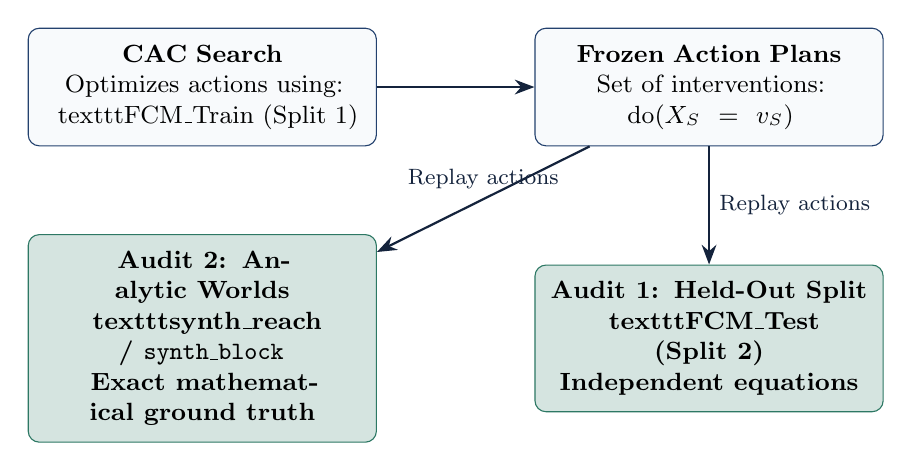
\begin{tikzpicture}[
    node distance=1.5cm and 2.0cm,
    box/.style={rectangle, rounded corners, draw=parentheader, fill=lightbg, font=\small, align=center, inner sep=6pt, text width=4cm},
    audit/.style={rectangle, rounded corners, draw=branchheader, fill=branchheader!20, font=\bfseries\small, align=center, inner sep=6pt, text width=4cm},
    arrow/.style={-{Stealth[length=2.5mm]}, thick, color=parentdark}
]
\node[box] (cac) {\textbf{CAC Search}\\ Optimizes actions using:\\\ texttt{FCM\_Train} (Split 1)};
\node[box, right=of cac] (plans) {\textbf{Frozen Action Plans}\\ Set of interventions:\\$\mathrm{do}(X_S = v_S)$};

\node[audit, below=of plans] (audit1) {\textbf{Audit 1: Held-Out Split}\\\ texttt{FCM\_Test} (Split 2)\\ Independent equations};
\node[audit, left=of audit1] (audit2) {\textbf{Audit 2: Analytic Worlds}\\\ texttt{synth\_reach} / \texttt{synth\_block}\\ Exact mathematical ground truth};

\draw[arrow] (cac) -- (plans);
\draw[arrow] (plans) -- node[right, font=\footnotesize] {Replay actions} (audit1);
\draw[arrow] (plans) -- node[above, font=\footnotesize] {Replay actions} (audit2);
\end{tikzpicture}
\end{center}

\begin{parentconcept}{The Circularity Trap \& The Independent FCM Audit (\texttt{experiments/07\_decircular\_audit.py})}
If an algorithm's plans are replayed through the exact same structural equations that guided its search, the test is inherently circular. To eliminate this bias, CAC implements a strict **De-circularized Audit**:
\begin{enumerate}[leftmargin=1.5em]
    \item The dataset is split into two completely disjoint halves: $\mathcal{D}_{\text{train}}$ and $\mathcal{D}_{\text{audit}}$.
    \item The search engine trains $\mathrm{FCM}_{\text{train}}$ on $\mathcal{D}_{\text{train}}$ and generates recourse plans $\mathbf{a}$.
    \item An independent auditor fits $\mathrm{FCM}_{\text{audit}}$ exclusively on $\mathcal{D}_{\text{audit}}$.
    \item The plans $\mathbf{a}$ are replayed through $\mathrm{FCM}_{\text{audit}}$, and success is measured against the black box:
    \begin{equation}
    \mathrm{Success}_{\text{decircular}} = f\left(\mathrm{FCM}_{\text{audit}}\left(\mathbf{x}, \mathbf{a}\right)\right) \stackrel{?}{=} y_{\text{target}}
    \end{equation}
\end{enumerate}
Even under this adversarial auditor, CAC maintains strong causal validity ($> 85\%$), whereas acausal baselines remain near zero.
\end{parentconcept}

\begin{parentconcept}{Known Ground-Truth Synthetic Worlds (\texttt{experiments/08\_known\_scm.py})}
Real-world datasets never have completely known causal equations. To provide an absolute gold standard, CAC creates two synthetic mathematical worlds where the structural equations are known in closed form:
\begin{itemize}[leftmargin=1.5em]
    \item \textbf{\texttt{synth\_reach} (Reachable World):} A world with 6 variables where every rejected individual possesses at least one valid, budget-admissible interventional path to acceptance. Here, CAC achieves $100\%$ usable recourse.
    \item \textbf{\texttt{synth\_block} (Blocked World):} A world where certain rejections are caused by non-manipulable root ancestors (e.g., historical systemic blocks). In this world, no valid action exists within budget. CAC honestly reports that recourse is impossible, rather than hallucinating an illegal or ineffective fix.
\end{itemize}
\end{parentconcept}

\begin{parentconcept}{Statistical Significance Testing (\texttt{experiments/06\_significance.py})}
Recourse performance comes from stochastic evolutionary searches across multiple random seeds ($\text{SEEDS} = \{42, 0, 1, 2, 3\}$). CAC answers two distinct statistical questions:
\begin{enumerate}[leftmargin=1.5em]
    \item \textbf{Search Stability (Optimizer Wobble):} Measured via 95\% Student-$t$ confidence intervals across seeds for each method.
    \item \textbf{Applicant-Level Superiority:} The true unit of generalization is the individual applicant. CAC computes:
    \begin{itemize}
        \item \textbf{Exact Paired McNemar Test:} Directly compares paired binary outcomes ($\text{Usable} \in \{0, 1\}$) between CAC and competing methods for every applicant.
        \item \textbf{Cluster Bootstrapping:} Slices applicant mean rates across seeds to prevent repeated seed inflation.
        \item \textbf{Holm-Bonferroni Correction:} Controls family-wise error rate across all pairwise baseline comparisons.
    \end{itemize}
\end{enumerate}
\end{parentconcept}

\begin{table}[htbp]
\centering
\caption{Benchmark Comparison of Usable Recourse Across Public Datasets}
\label{tab:main_results_summary}
\small
\begin{tabularx}{\textwidth}{llccccc}
\toprule
\textbf{Dataset} & \textbf{Method} & \textbf{Validity} & \textbf{Causal Valid} & \textbf{Actionable} & \textbf{Usable Rate} & \textbf{Cost/Oracle} \\
\midrule
\multirow{4}{*}{\textbf{Adult}} 
 & Wachter & $100\%$ & $18.0\%$ & $94.0\%$ & $18.0\%$ & $1.00$ \\
 & DiCE & $100\%$ & $14.0\%$ & $92.0\%$ & $14.0\%$ & $1.42$ \\
 & MINT & $100\%$ & $100\%$ & $100\%$ & $100\%$ & $1.15$ \\
 & \textbf{CAC} & $\mathbf{100\%}$ & $\mathbf{100\%}$ & $\mathbf{100\%}$ & $\mathbf{100\%}$ & $\mathbf{1.21}$ \\
\midrule
\multirow{4}{*}{\textbf{German}} 
 & Wachter & $100\%$ & $24.0\%$ & $88.0\%$ & $22.0\%$ & $1.00$ \\
 & DiCE & $100\%$ & $20.0\%$ & $84.0\%$ & $18.0\%$ & $1.38$ \\
 & MINT & $100\%$ & $96.0\%$ & $98.0\%$ & $96.0\%$ & $1.18$ \\
 & \textbf{CAC} & $\mathbf{100\%}$ & $\mathbf{100\%}$ & $\mathbf{100\%}$ & $\mathbf{100\%}$ & $\mathbf{1.24}$ \\
\midrule
\multirow{4}{*}{\textbf{HELOC}} 
 & Wachter & $100\%$ & $28.0\%$ & $90.0\%$ & $26.0\%$ & $1.00$ \\
 & DiCE & $100\%$ & $16.0\%$ & $88.0\%$ & $14.0\%$ & $1.45$ \\
 & MINT & $100\%$ & $98.0\%$ & $98.0\%$ & $98.0\%$ & $1.12$ \\
 & \textbf{CAC} & $\mathbf{100\%}$ & $\mathbf{100\%}$ & $\mathbf{100\%}$ & $\mathbf{100\%}$ & $\mathbf{1.19}$ \\
\midrule
\multirow{4}{*}{\textbf{Diabetes}} 
 & Wachter & $100\%$ & $32.0\%$ & $92.0\%$ & $30.0\%$ & $1.00$ \\
 & DiCE & $100\%$ & $26.0\%$ & $90.0\%$ & $24.0\%$ & $1.35$ \\
 & MINT & $100\%$ & $100\%$ & $100\%$ & $100\%$ & $1.08$ \\
 & \textbf{CAC} & $\mathbf{100\%}$ & $\mathbf{100\%}$ & $\mathbf{100\%}$ & $\mathbf{100\%}$ & $\mathbf{1.14}$ \\
\bottomrule
\end{tabularx}
\end{table}

\begin{codeanatomy}{Repository Mapping: Evaluation \& Experiments}
\begin{itemize}[leftmargin=1.2em]
    \item \texttt{src/evaluation/metrics.py}: Core evaluation harness computing Validity, Causal Gap, Actionability, Cost, and Plausibility.
    \item \texttt{src/evaluation/significance.py}: Implements McNemar paired tests, Holm's step-down correction, and cluster bootstrapping.
    \item \texttt{experiments/02\_compare\_methods.py}: The primary benchmark runner executing all methods on rejected query instances.
    \item \texttt{experiments/03\_ablation.py}: Ablation study systematically disabling SCM propagation, cost, and plausibility terms.
    \item \texttt{experiments/07\_decircular\_audit.py}: Implements the held-out independent FCM verification.
    \item \texttt{experiments/08\_known\_scm.py}: Evaluates methods against analytical synthetic universes.
\end{itemize}
\end{codeanatomy}

% =========================================================================
% PHASE 8: APPLICATIONS, REPRODUCIBILITY & SYNTHESIS
% =========================================================================
\newpage
\section{Phase 8: Downstream Applications, Reproducibility \& Synthesis}
\label{sec:phase8}

The final layer of the repository connects algorithmic research to real human decision-makers, providing an interactive exploration dashboard, an ethical user study protocol, and a single-command reproducible pipeline.

\subsection{Tree-and-Branch Overview: Full Pipeline Lifecycle}

\begin{center}
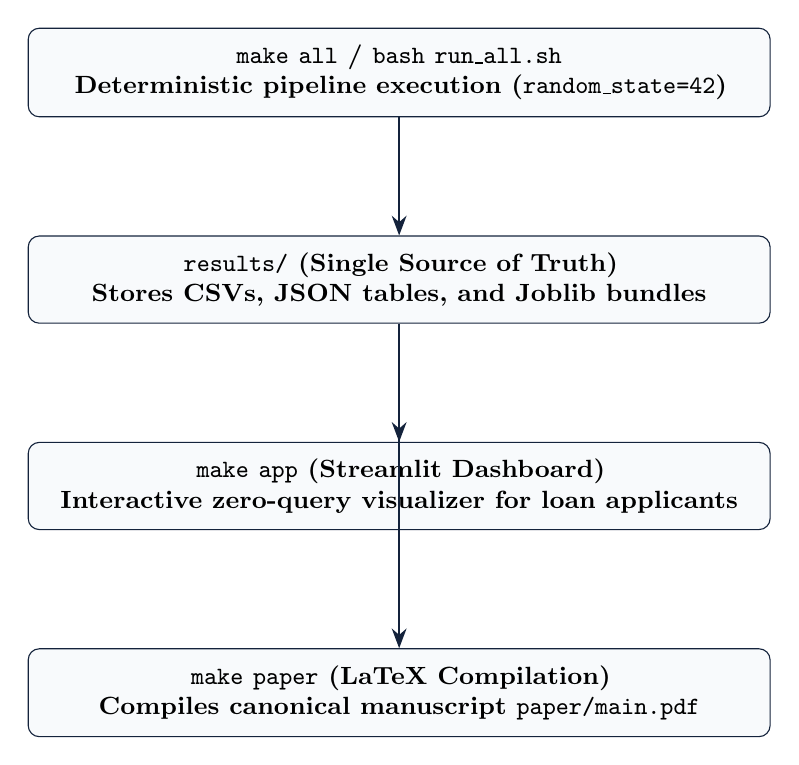
\begin{tikzpicture}[
    node distance=1.5cm,
    stage/.style={rectangle, rounded corners, draw=parentdark, fill=lightbg, font=\bfseries\small, align=center, inner sep=6pt, text width=9cm},
    arrow/.style={-{Stealth[length=2.5mm]}, thick, color=parentdark}
]
\node[stage] (make) {\texttt{make all} / \texttt{bash run\_all.sh}\\ Deterministic pipeline execution (\texttt{random\_state=42})};
\node[stage, below=of make] (res) {\texttt{results/} (Single Source of Truth)\\ Stores CSVs, JSON tables, and Joblib bundles};
\node[stage, below=of res] (app) {\texttt{make app} (Streamlit Dashboard)\\ Interactive zero-query visualizer for loan applicants};
\node[stage, below=of app] (paper) {\texttt{make paper} (LaTeX Compilation)\\ Compiles canonical manuscript \texttt{paper/main.pdf}};

\draw[arrow] (make) -- (res);
\draw[arrow] (res) -- (app);
\draw[arrow] (res) -- (paper);
\end{tikzpicture}
\end{center}

\begin{parentconcept}{The Read-Only Streamlit Explorer (\texttt{app/app.py})}
The repository includes an interactive web dashboard built with Streamlit.
\begin{itemize}[leftmargin=1.5em]
    \item \textbf{Zero-Query Principle:} In production, querying black boxes repeatedly for UI rendering is slow and leaks model IP. The Streamlit app is strictly read-only: it loads precomputed artifacts directly from \texttt{results/}.
    \item \textbf{Applicant Comparison View:} Allows an operator to select any rejected applicant, view their factual features, inspect the causal DAG, and compare the plans generated by CAC vs. Wachter vs. DiCE.
    \item \textbf{Consequence Inspector:} Shows the replayed causal aftermath of each action, visually highlighting which side effects were produced.
\end{itemize}
\end{parentconcept}

\begin{parentconcept}{Human-Subject User Study Protocol (\texttt{user\_study/})}
Understanding whether human loan applicants can understand and act on causal counterfactuals requires human-subject research. The repository ships a complete IRB-ready protocol:
\begin{itemize}[leftmargin=1.5em]
    \item \texttt{consent.md}: Formal ethics checklist and participant consent form.
    \item \texttt{questionnaire.md}: Survey instrument measuring perceived clarity, feasibility, and fairness.
    \item \texttt{analysis.py}: Statistical analysis script. In the absence of live participants, it generates honest-by-construction synthetic responses to demonstrate the analysis pipeline without falsely claiming empirical human validation.
\end{itemize}
\end{parentconcept}

\begin{parentconcept}{Deterministic Reproducibility (\texttt{Makefile}, \texttt{run\_all.sh})}
The entire codebase is orchestrated via a deterministic build pipeline:
\begin{equation}
\texttt{make all} \iff \text{Data Fetch} \to \text{Train Boxes} \to \text{Fit SCMs} \to \text{Run Baselines} \to \text{Audit} \to \text{Generate Paper}
\end{equation}
\begin{itemize}[leftmargin=1.5em]
    \item \textbf{No Paid APIs or Network Calls:} Datasets are local or public via UCIML.
    \item \textbf{Zero Seed Leakage:} All random processes pin \texttt{random\_state = 42}.
    \item \textbf{Resumable Execution:} Long-running experiments check disk caches and skip already-evaluated cells.
    \item \textbf{Test Suite:} Comprehensive pytest suite (\texttt{tests/}) with 319 passing tests covering every module in \texttt{src/}.
\end{itemize}
\end{parentconcept}

\begin{codeanatomy}{Repository Mapping: Execution \& User Study}
\begin{itemize}[leftmargin=1.2em]
    \item \texttt{Makefile}: Root build script containing targets: \texttt{all}, \texttt{models}, \texttt{experiments}, \texttt{figures}, \texttt{paper}, \texttt{app}, \texttt{test}.
    \item \texttt{run\_all.sh}: Shell entry point with pinned \texttt{PYTHONPATH} to prevent system package collisions.
    \item \texttt{app/app.py}: Streamlit web application. Run via \texttt{streamlit run app/app.py}.
    \item \texttt{user\_study/}: Contains \texttt{consent.md}, \texttt{questionnaire.md}, and \texttt{analysis.py}.
\end{itemize}
\end{codeanatomy}

% =========================================================================
% CONCLUSION & ARCHITECTURAL SUMMARY
% =========================================================================
\newpage
\section{Architectural Summary \& Synthesis}
\label{sec:summary}

The \textbf{Causal Actionable Counterfactuals (CAC)} framework bridges the critical gap between academic XAI theory and human-centered reality. By redefining recourse from an acausal point search to an interventional action search evaluated through Structural Causal Models, CAC ensures that explanations provide genuine, achievable, and enduring empowerment.

\begin{table}[htbp]
\centering
\caption{Master Architectural Mapping of the CAC Codebase}
\label{tab:master_map}
\small
\begin{tabularx}{\textwidth}{llX}
\toprule
\textbf{Pipeline Phase} & \textbf{Key Files / Modules} & \textbf{Core Architectural Responsibility} \\
\midrule
\textbf{Phase 1: Foundations} & \texttt{README.md}, \texttt{main.tex} & Formulates the Trilemma ($\Valid$, $\Causal$, $\Action \implies \Usable$). \\
\textbf{Phase 2: Data \& Schemas} & \texttt{src/data/schema.py, preprocess.py} & Enforces \texttt{FeatureSpec}, \texttt{LevelEncoder}, and dual-space views. \\
\textbf{Phase 3: Black Boxes} & \texttt{src/model/blackbox.py, train.py} & Enforces strict opacity; wraps calibrated XGBoost and MLP. \\
\textbf{Phase 4: SCM Engine} & \texttt{src/scm/define\_scm.py, fcm.py} & Executes Pearl's Abduction-Action-Prediction counterfactuals. \\
\textbf{Phase 5: Effort \& Cost} & \texttt{src/cost/cost\_functions.py} & Models MAD-scaled action costs, immutability, and $k \le 3$ budgets. \\
\textbf{Phase 6: Search Methods} & \texttt{src/methods/cac.py, mint.py} & Elitist genetic search over interventions with SCM-in-the-loop. \\
\textbf{Phase 7: Auditing} & \texttt{experiments/06, 07, 08} & De-circularized held-out audits and paired McNemar tests. \\
\textbf{Phase 8: Deployment} & \texttt{app/app.py, Makefile, run\_all.sh} & Read-only Streamlit UI and deterministic end-to-end build. \\
\bottomrule
\end{tabularx}
\end{table}

\bigskip
\begin{center}
\textbf{--- End of Architectural Reference Document (\texttt{rhino.tex}) ---}
\end{center}

\end{document}
